\documentclass[12pt,a4paper]{article}
\usepackage{adjustbox} % in preamble

\usepackage[utf8]{inputenc}
\usepackage[latvian]{babel}
\usepackage{caption}
\usepackage{hyperref}

% Make captions "1. attēls."
\DeclareCaptionLabelFormat{numberfirst}{\arabic{figure}. attēls}
\captionsetup[figure]{labelformat=numberfirst,labelsep=period}

% Command for referencing: "1. attēls"
\newcommand{\figref}[1]{\ref{#1} attēls}


\pagenumbering{arabic} % Sets page numbering to arabic (1, 2, 3, ...)
\setcounter{page}{1} % Specifies the starting page number

\usepackage{tabularx} % in your preamble
\usepackage{amsmath, amssymb}
\usepackage{graphicx}
\usepackage{geometry}
\usepackage{subcaption}
\usepackage{float}
\usepackage{array}
\usepackage{booktabs}
\usepackage{enumitem}
\usepackage{fancyhdr}
\usepackage{xcolor}
\usepackage{framed}
\usepackage{titlesec}
\usepackage{subcaption}

% Example 1: Bold, larger font, with some vertical spacing
\titleformat{\section}
  {\normalfont\Large\bfseries} % format: font + weight
  {\thesection}                % label (number)
  {0.3em}                         % space between number and title
  {}                            % code before title text

\geometry{
    left=2cm,
    right=2cm,
    top=2.5cm,
    bottom=2.5cm
}

\pagestyle{plain}
\fancyhf{}
\rhead{Olbaltumvielas}

% Custom colors and environments
\definecolor{taskbg}{rgb}{0.95,0.95,0.95}

% Custom environment for tasks
\newenvironment{taskbox}
{\begin{framed}\begin{minipage}{\textwidth}}
{\end{minipage}\end{framed}}

\title{\textbf{Olbaltumvielas}}
\author{}
\date{}

\begin{document}

\maketitle

    Vai esi kādreiz aizdomājies/usies par to, kā cilvēks un citi organismi spēj izpildīt tik kompleksas funkcijas ar tik šķietami vienkāršām struktūrām? Kā mēs nodrošinām specifiskas ķīmiskās reakcijas, transportējam vielas, saraujam muskuļus, pasargājamies no infekcijas un pārvadām signālus no vienas ķermeņa daļas uz citu? Patiesībā atbilde uz visiem šiem jautājumiem slēpjas vienā vārdā — olbaltumvielas! Taču kas tie ir un ko tie dara? Lai atbildētu uz šiem jautājumiem un atvieglinātu darbu olimpiādē, iepazīsties tālāk ar šo fascinējošo molekulu grupu, izlasot doto informāciju un izpildot testa jautājumus!


\section{Aminoskābju uzbūve un īpašības}

Kā jau tika minēts, olbaltumvielas jeb proteīni ir molekulas, bez kurām dzīvība nespētu esksitēt jebkādā mērā. Tie ir polimēri, kas sastāv no $\alpha$-aminoskābju atlikumiem. Organismu šūnās tie rodas gēnu ekspresijas ceļā, transkribējot DNS par RNS un translējot RNS par olbaltumvielu. Šo procesu sauc par \textbf{centrālo dogmu}.

Aminoskābes (olbaltumvielu monomēri) ir oglekļa ķēdes ar karbonskābes un aminogrupu galos. Olbaltumvielas sastāv no $\alpha$-aminoskābēm, kuru atlikuma sastāvā ir tikai divi oglekļa atomi, kur $\alpha$-ogleklim pievienota specifiska sānu ķēde (R). Šīs sānu ķēdes uzbūve nosaka aminoskābes veidu, savukārt aminoskābju secība — olbaltumvielas uzbūvi un īpašības.

Cilvēku ķermenī kopā pastāv 22 aminoskābju veidi, taču mūsu gēni kodē tikai 20 vislabāk pazīstamās aminoskābes. Katra veida sānu ķēde nosaka izmēru, formu, šķīdību un jonizāciju. Aminoskābes tālāk var iedalīt nepolārās, polārās, pozitīvi un negatīvi lādētās (\figref{fig:aminoskabes})

\begin{figure}[H]
    \centering
    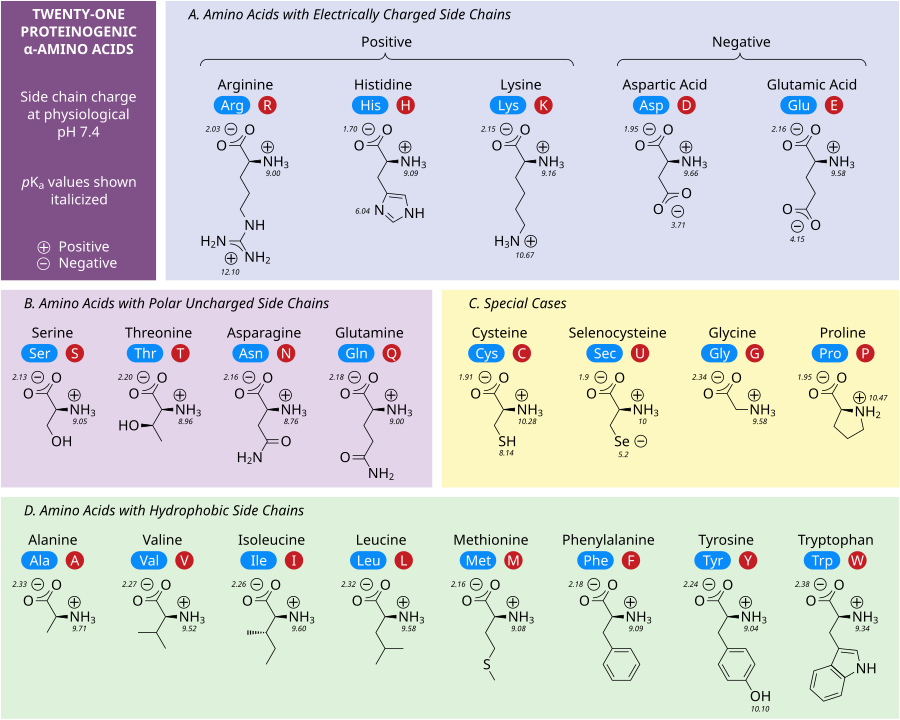
\includegraphics[width=0.5\textwidth]{atteli/proteīni-1.png}
    \caption{Aminoskābju iedalījums pēc polaritātes un lādiņa.}
    \label{fig:aminoskabes}
\end{figure}

Tā kā aminoskābes veidojas enzimātisku reakciju ceļā, sintezējamās aminoskābes nosaka organisma suga. Cilvēks ir pats spējīgs sintezēt lielāko daļu aminoskābju, atliek tikai deviņas, kuras obligāti jāuzņem caur uzturu. 

\begin{table}[H]
\centering
\begin{tabularx}{\textwidth}{|
    >{\raggedright\arraybackslash}p{4.5cm}|
    >{\raggedright\arraybackslash}X|}
\hline
Neaizstājamās aminoskābes &
Histidīns, izoleicīns, leicīns, metionīns, fenilalanīns, treonīns, triptofāns, valīns \\
\hline
Aizstājamās aminoskābes &
Alanīns, arginīns, asparagīns, aspargīnskābe, cisteīns, glutamīnskābe,
glutamīns, glicīns, prolīns, selenocisteīns, serīns, tirozīns \\
\hline
\end{tabularx}
\end{table}


Par īpašu uzskatāma aminoskābju spēja veidot vienlaicīgi pozitīvi un negatīvi lādētas daļiņas jeb dipolārus jonus. Molekulas ar pozitīvi un negatīvi lādētiem apgabaliem dēvē par \textbf{cviterjoniem}. Nereti, pierakstot aminoskābes, tiek izmantota cviterjonu forma, atņemot protonu no karbonskābes grupas un pievienojot to aminogrupai (respektīvi veidojot negatīvu un pozitīvu lādiņu šajos molekulas galos). Šo formu stabilizē šķīdinātājs (parasti ūdens) un jonu veidošanos nosaka vides pH. Skābos apstākļos karbonskābes grupai tiek pievienots protons, aminoskābei kļūstot pozitīvi lādētai, savukārt bāziskos apstākļos no aminogrupas tiek atņemt protons, molekulai gūstot negatīvu lādiņu (\figref{fig:cviterjoni}).

\begin{figure}[H]
    \centering
    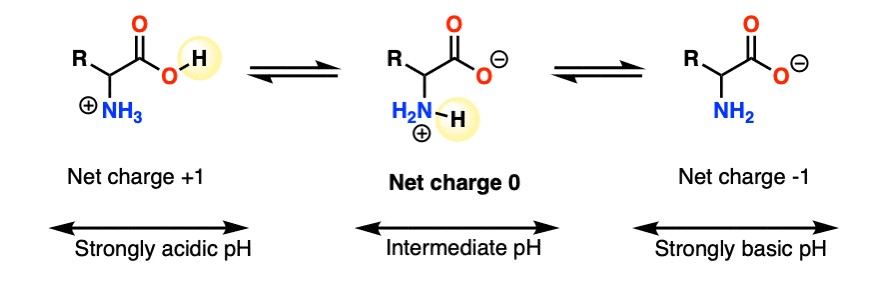
\includegraphics[width=0.5\textwidth]{atteli/proteīni 2.jpg}
    \caption{Aminoskābes cviterjona pārvērtības atkarībā no vides pH.}
    \label{fig:cviterjoni}
\end{figure}

\section{Olbaltumvielu strukturālie līmeņi}

Uzzinot par aminoskābēm — olbaltumvielu sastāvdaļām, loģiski izriet jautājums par to kā tās savienojas, kā veidojas olbaltumviela. Tas notiek kondensācijas polimerizācijas reakcijā, vairākām aminoskābēm savienojoties ar \textbf{peptīdsaiti} (\figref{fig:peptidsaite}), lai veidotu peptīdu vai polipeptīdu. Divas aminoskābes veido dipeptīdu, trīs — tripeptīdu utt. Ja ķēdes garums pārsniedz 50 aminoskābes, iegūto molekulu sauc par \textbf{polipeptīdu}, tātad olbaltumvielu.


\begin{figure}[H]
    \centering
    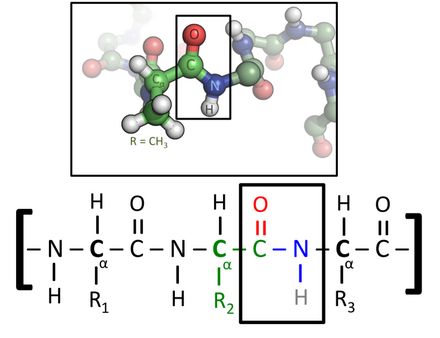
\includegraphics[width=0.3\textwidth]{atteli/proteīni 3.png}
    \caption{Peptīdsaites struktūrformula.}
    \label{fig:peptidsaite}
\end{figure}


Tātad, aminoskābēm savienojoties veidojas polipeptīda ķēde. To bioloģijā dēvē par olbaltumvielas \textbf{pirmējo struktūru} (\figref{fig:strukturas}). Vienā ķēdes galā eksistē aminogrupa, bet otrā — karbonskābes grupa. Šos galus respektīvi sauc par N-terminālo galu un C-terminālo galu. Tas nozīmē, ka katram polipeptīdam iespējams noteikt sākumu un galu, vadoties no N-terminālā gala uz karbonskābes grupu.

Ko tagad? Visas olbaltumvielas šūnā ieņem telpisku formu, taču polimerizācijas reakcijā iegūtajai ķēdei ir lineāra ģeometrija. Izrādās, ka aminoskābju atlikumiem savstarpējā mijiedarbībā (starp skābekļa un ūdeņraža atomiem) rodas vājas ūdeņražsaites, kas piešķir dažādām polipeptīda daļām atšķirīgu formu. Struktūras, kas veidojas šajā procesā iedala alfa spirālēs un beta plātnēs, šo uzbūves līmeni sauc par \textbf{otrējo struktūru}.

Nākamās mijiedarbojas aminoskābju sānu ķēdes, veidojot olbaltumvielas \textbf{trešējo struktūru}. Šeit iespējamas dažādas saites un spēki, katrai ietekmējot olbaltumvielas struktūru atšķirīgos veidos. Piemēram, starp divām cisteīna sānu ķēdēm var veidoties disulfīda tiltiņš, kovalenti saistot dažādas polipeptīda lokācijas un ieliecot molekulu. Vēl starp sānu ķēdēm var veidoties joniskas saites, ūdeņražsaites un hidrofobas mijiedarbības. Olbaltumvielas trešējo struktūru var iedalīt daudzos veidos, bet pamatā tie ir globulāri (sfēriski) vai fibrilāri (gareni, lineāri).

Visaugstākā olbaltumvielu struktūra nav universāla, bet gan veidojas savienojoties vairākiem polipeptīdiem vienā molekulā. Olbaltumvielas, kas sastāv no vairākām aminoskābju ķēdēm sauc par \textbf{ceturtējās struktūras} olbaltumvielām. Piemērs ceturtējās struktūras olbaltumvielai ir hemoglobīns, kurš sastāv no 4 polipeptīdiem, katram ar savu skābekli vai ogļskābo gāzi piesaistošo hēma grupu.

\begin{figure}[H]
    \centering
    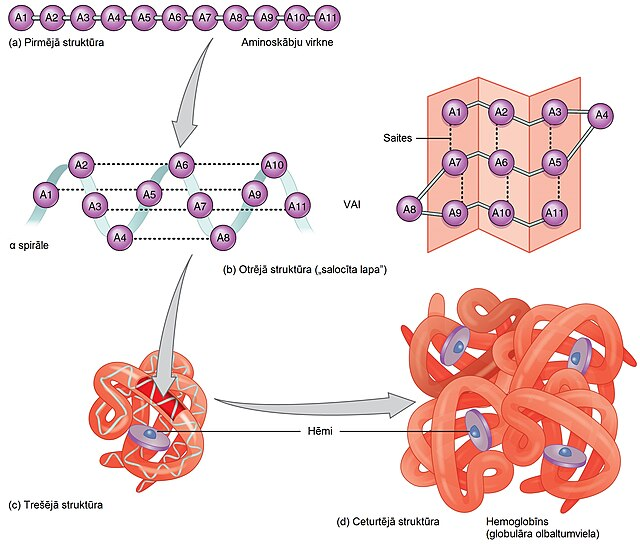
\includegraphics[width=0.5\textwidth]{atteli/proteīni 4.jpg}
    \caption{Olbaltumvielas uzbūves līmeņi.}
    \label{fig:strukturas}
\end{figure}

\section{Denaturācija}
Olbaltumvielu struktūra ir atkarīga arī no apkārtējās vides, un, ja tā atšķiras no olbaltumvielai nepieciešamās, tad ķīmiskās saites olbaltumvielā var tikt izjauktas, sabojājot tās struktūru. Šis process, kurā olbaltumviela ārējo apstākļu ietekmē zaudē savu formu un līdz ar to arī savu funkcionalitāti, sauc par denaturāciju. Tā var notikt ķīmisko faktoru ietekmē, piemēram, pārāk skābā vai pārāk bāziskā vidē, vai arī smago metālu sāļu ietekmē. Olbaltumvielas iekšpusi veido hidrofobas aminoskābes, bet ārpusi — hidrofilas, tāpēc, ievietojot olbaltumvielu hidrofobā vidē, tā denaturējas, jo tās iekšas vēlas "izgrozīties" uz ārpusi. Denaturāciju var izraisīt arī fiziskie faktori, tādi kā dažāda veida starojumi, piemēram, UV starojums, pārāk liela temperatūra (lielāka par 50 grādiem), kā arī stipras vai ilgstošas vibrācijas. Denaturācija var būt atgriezeniska, kad, apstākļiem atgriežoties pie normāliem, olbaltumviela atgūst savu formu (šo procesu sauc par renaturāciju), vai neatgriezeniska, kad struktūra vairs nav atjaunojama.

\section{Olbaltumvielu funkcijas}

Dabā pastāv neskaitāmi daudz olbaltumvielu, un zinātnieki turpina atklāt jaunas. Katrai olbaltumvielai ir sava specifiska forma un funkcija. Tām ir daudz uzdevumu, kas ir iesaistīti visos šūnu procesos. Enzimātisko olbaltumvielu funkcija ir ķīmisko reakciju veicināšana šūnā, piemēram, gremošanas enzīms laktāze sašķeļ disaharīdu laktozi par diviem monosaharīdiem — glikozi un galaktozi. Citām olbaltumvielām ir vielu uzglabāšanas funkcija. Piemēram, ovalbumīns, kuru satur olas, ir aminoskābju avots priekš embrija. Olbaltumvielas pilda aizsardzības funkciju, piemēram antigēni pievienojas vīrusiem, padarot tos redzamus šūnām, kuras tos iznīcina, un, turklāt, neļaujot pievienoties šūnu receptoriem un iebrukt tajās. Ir olbaltumvielas, piemēram, hemoglobīns, kuras pilda vielu transporta funkciju. Membrānu olbaltumvielas nodrošina vielu transportu uz šūnu un no tās. Olbaltumvielas atbild arī par organisma darbības regulāciju, pildot gan hormonu, gan receptoru funkcijas. Viens no hormoniem, kurš ir olbaltumviela, ir insulīns. Olbaltumvielas nodrošina kustību, jo no tiem sastāv cilvēka miofilamenti, kuri veic muskuļu saraušanos. Turklāt, olbaltumvielas veic strukturālo funkciju. Piemēram, no keratīna sastāv cilvēku nagi un mati.


\section{Olbaltumvielas un mutācijas}

Olbaltumvielas ir arī cieši saistītas ar ģenētisko informāciju, kas kodē aminoskābju sekvenci šajā olbaltumvielā. Ja ģenētiskajā kodā notikušas kādas izmaiņas — mutācijas, tad sagaidāms, ka arī olbaltumvielas struktūra būs mainīta. Ir dažādi mutāciju veidi, piemēram, punktveida mutācijas, hromosomu aberāciajs un hromosomu skaita izmaiņas.

Mutāciju sauc par punktveida mutāciju, ja izmaiņas notikušas vienā nukleotīdā. Tieši šīs mutācijas parasti visbiežāk ietekmē olbaltumvielu pirmējo struktūru. Kā redams \ref{fig:mutacijas} attēlā, punktveida mutāciju ietekme uz olbaltumvielu pirmējo struktūru var būt dažāda. Viens no veidiem ir klusā mutācija, kad, lai gan ir DNS sekvencē ir notikusi substitūcija (viens nukleotīds nomainīts pret citu), šī tripleta kodētā aminoskābe nemainās, tātad arī olbaltumvielā nav izmaiņu. Missense mutāciju gadījumā DNS triplets kodē citu aminoskābi, nekā iepriekš. Tas, cik ļoti notikusī izmaiņa ietekmē olbaltumvielu struktūru un spēju veikt funkcijas atkarīgs no tā, cik līdzīga ir aizvitotā aminoskābe, kā arī cik svarīga tā ir olbaltumvielas darbībā. Nonsense mutācija ir tad, kad DNS kodons, kas iepriekš kodēja aminoskābi, tagad kodē STOP kodonu. Šajos gadījumos tiek priekšlaicīgi pārtraukta translācija un tas, cik ļoti ietekmēta olbaltumvielas struktūra un darbība atkarīgs, cik tuvu vai tālu no sākotnējā stop kodona notikusi mutācija. Gadījumos, ja notikusi insercija (nukleotīda ieveitošana) vai delēcija (nukleotīda zaudēšana), var notikt translācijas fāzes nobīde (frameshift angļu valodā), kā rezultātā ir izmainīta ne tikai aminoskābe, kuras kodonā notikusi mutācija, bet arī visas pārējās aminoskābes pēc tās.

\begin{figure}[H]
    \centering
    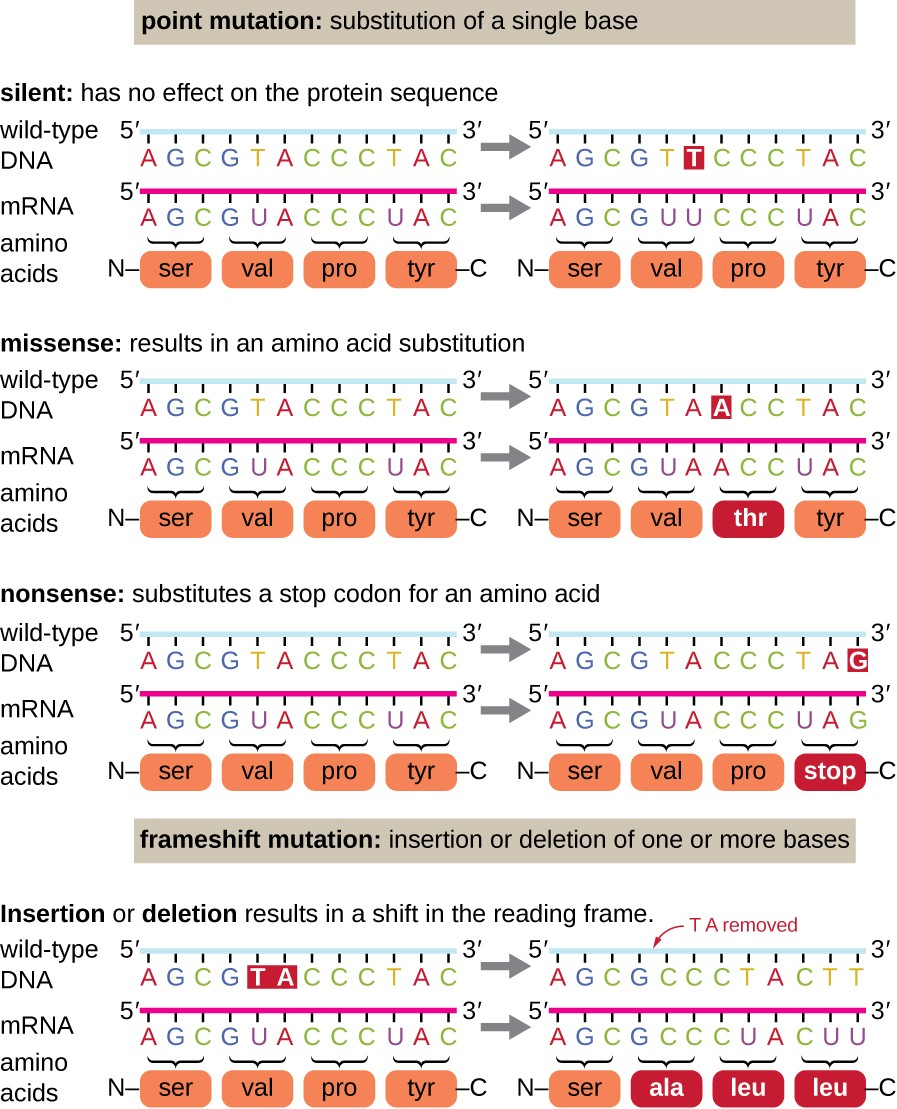
\includegraphics[width=0.5\textwidth]{atteli/mutācijas-1.jpg}
    \caption{Punktveida mutāciju veidi.}
    \label{fig:mutacijas}
\end{figure}

\section*{Jautājumi}

\noindent \textbf{1. jautājums.} Kādi monomēri savienojas, veidojot polipeptīdus?

\begin{enumerate}[label=\Alph*.]
    \item vienkārši cukuri
    \item lipīdi
    \item nukleīnskābes
    \item aminoskābes
    \item taukskābes
\end{enumerate}


\begin{figure}[h]
    \centering
    \begin{minipage}[c]{0.55\textwidth} % Left side: question
        \textbf{2. jautājums.} Kāda funkcionālā grupa trūkst \ref{fig:grupa} attēlā redzamajai aminoskābei?

        \begin{enumerate}[label=\Alph*.]
            \item COOH
            \item NH
            \item CH
            \item SH
            \item OH
        \end{enumerate}
    \end{minipage}%
    \hfill
    \begin{minipage}[c]{0.40\textwidth} % Right side: image
        \centering
        \adjustbox{valign=c}{%
            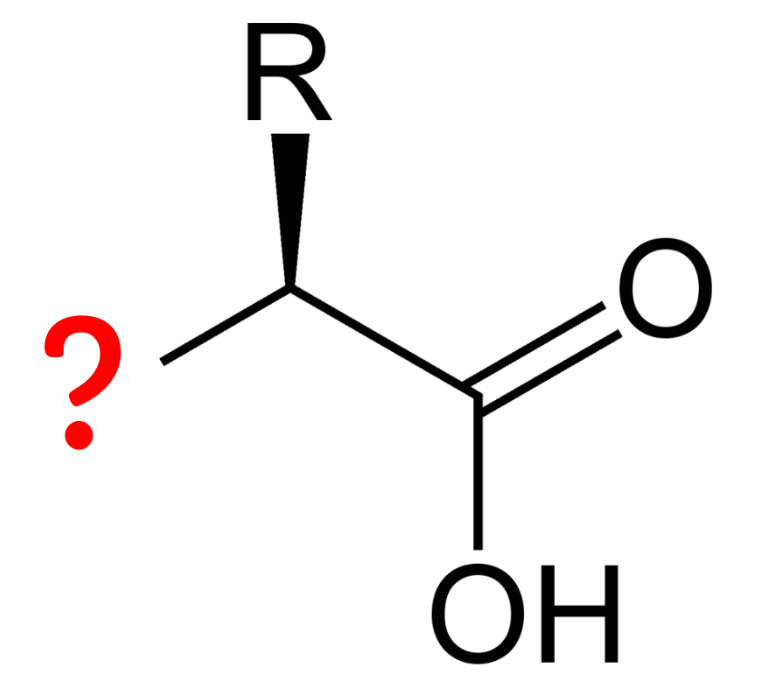
\includegraphics[width=0.7\textwidth]{atteli/aminoskabe.png}}
        \caption{~}
        \label{fig:grupa}
    \end{minipage}
\end{figure}


\noindent \textbf{3. jautājums.} Kurš variants visprecīzāk apraksta ūdeņražsaišu lomu olbaltumvielu uzbūvē?

\begin{enumerate}[label=\Alph*.]
    \item  Ūdeņražsaites veidojas starp aminoskābēm, lai veidotu alfa spirāles un beta plātnes. 
    \item Ūdeņražsaites veidojas aminoskābēs, lai savienotu karboksilgrupu ar aminogrupu.
    \item Starp aminoskābēm veidojas ūdeņražsaites, lai veidotu polipeptīdu ķēdi.
    \item Ūdeņražsaites nodrošina olbaltumvielu polimerizāciju.
\end{enumerate}

\noindent \textbf{4. jautājums.} Kurš no šiem apgalvojumiem raksturo olbaltumvielu otrējo struktūru?

\begin{enumerate}[label=\Alph*.]
    \item Sarežģīta 3D struktūra, kas veidojas, mijiedarbojoties un apvienojoties vairākiem polipeptīdiem.
    \item 3D struktūra, kas veidojas aminoskābju sānu ķēdes mijiedarbības dēļ.
    \item Aminoskābju secība polipeptīdu ķēdē.
    \item Salocīta struktūra, ko veido ūdeņražsaites, kas veidojas starp aminoskābju atlikumiem.

\end{enumerate}


\begin{figure}[h]
    \centering
    % Left: question
    \begin{minipage}[c]{0.55\textwidth}
        \textbf{5. jautājums.} Izmantojot valīna un glutamīnskābes struktūrformulas \ref{fig:valins_glutamins} attēlā, nosaki kāda veida mijiedarbības norisināsies to saturošas olbaltumvielas trešējā struktūrā!
        
        \begin{enumerate}[label=\Alph*.]
            \item ūdeņražsaites
            \item jonu saites
            \item disulfīda tiltiņi
            \item hidrofobā mijiedarbība
            \item neveidosies spēcīga mijiedarbība
        \end{enumerate}
    \end{minipage}%
    \hfill
    % Right: two subfigures
    \begin{minipage}[c]{0.40\textwidth}
        \centering
        \begin{subfigure}[c]{0.48\textwidth}
            \adjustbox{valign=c}{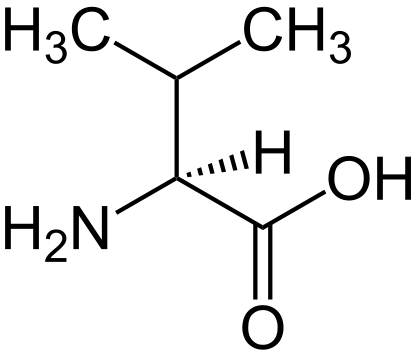
\includegraphics[width=\textwidth]{atteli/valins.png}}
            \caption{Valīns}
            \label{fig:valins}
        \end{subfigure}%
        \hfill
        \begin{subfigure}[c]{0.48\textwidth}
            \adjustbox{valign=c}{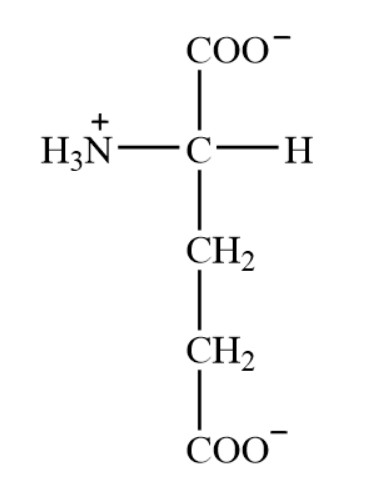
\includegraphics[width=\textwidth]{atteli/prot-glutamīnskābe.png}}
            \caption{Glutamīnskābe}
            \label{fig:glutamins}
        \end{subfigure}
        \caption{~}
        \label{fig:valins_glutamins}
    \end{minipage}
\end{figure}


\noindent \textbf{6. jautājums.} Kāda veida mutācija notikusi, ja olbaltumvielā tikai viena aminoskābe ir nomainīta pret citu?

\begin{enumerate}[label=\Alph*.]
    \item klusā mutācija
    \item missense mutācija
    \item nonsense mutācija
    \item insercija
    \item delēcija
\end{enumerate}


\section*{Atsauces}
\begin{enumerate}[leftmargin=*]
    \item Contributors to Wikimedia projects. \textit{Olbaltumvielas}. \url{https://lv.wikipedia.org/wiki/Olbaltumvielas}
    \item Urry, L. A.; Cain, M. L.; Wasserman, S. A.; Minorsky, P. V.; Orr, R. \textit{Campbell Biology}; 2020.
    \item \textit{Mutations | Microbiology}. \url{https://courses.lumenlearning.com/suny-microbiology/chapter/mutations/}
\end{enumerate}


\newpage
\section*{Atbildes}

\begin{enumerate}
\item D
\item B
\item A
\item D
\item E. Skaidrojums: valīna sānu ķēde ir hidrofoba, un glutamīnskābes sānu ķēde ir polāra. Starp šādām sānu ķēdēm nav specifisku mijiedarbību.
\item B
\end{enumerate}

\end{document}